\chapter{Point intensity transforms}
\lecture{3}{25/10}

Here we are looking at functions that take a pixel value $p$ and transforms them to another state $p'$
\[ p' = f(p). \]
$f$ is known as an \textbf{intensity transform function}.
The main application for this is \emph{image enhancement}.
The goal with image enhancement is to make an image look \emph{better} so we can process it with greater clarity;
however, it is clearly subjective what is better and depeneds on
\begin{enumerate}
    \item the information required from the image;
    \item the physical characteristics of the image;
    \item the user's prior knowledge and experience; and
    \item the user's intuition and judgement.
\end{enumerate}

Poor lighting and noise are some common \emph{poor} image characteristics.

\begin{definition}[Range]
    The \textbf{range} of a sensor is the set of all possible intensity values it can capture.
\end{definition}

A \emph{good} image should utilise most of a sensor's range.

\begin{definition}[Dynamic range]
    The \textbf{dynamic range} of a sensor, display, or image 
    is the largest (possible) signal divided by the smalled (possible) signal.
\end{definition}

We can increase the contrast of an image by increasing the dynamic range.

\section{Logarithmic transform}

A simple \textbf{logarithmic transform} replaces each pixel value with its logarithm:
\[ I_o(i,j) = \log{(I_i(i,j))}, \]
but in practise we introduce parameters $\sigma, c > 0$ to control the range:
\[ I_o(i, j) = c\log{\left(1 + (e^\sigma - 1)I_i(i, j)\right)}. \]
Figure \ref{fig:log-scaling-factor} demonstrates how $\sigma$ changes our transform.
We define $c$ to normalise our output range to (typically) 255, so
\[ c = \frac{255}{\max{(\log{(1 + (e^\sigma - 1)I_i(i, j))})}} \]

\begin{figure}
    \centering
    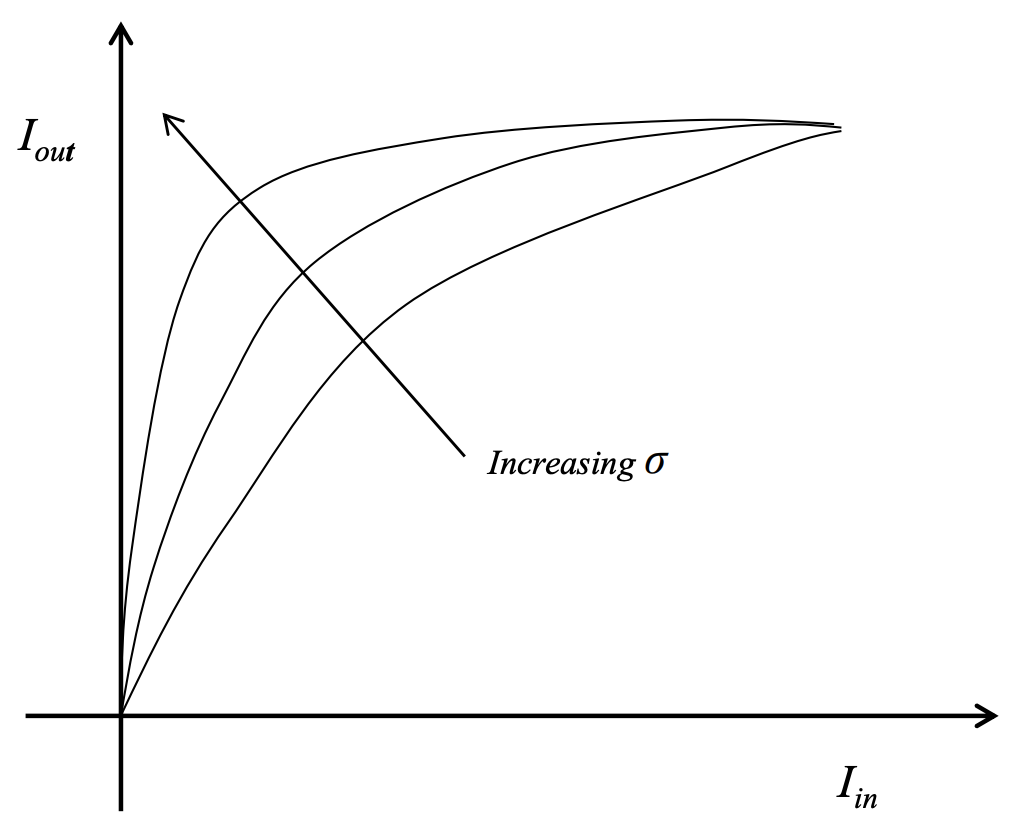
\includegraphics[width=0.5\linewidth]{images/log-scaling-factor.png}
    \caption{A graph demonstrating how a change in $\sigma$ affects the logarithmic transform.}
    \label{fig:log-scaling-factor}
\end{figure}

\begin{figure}
    \centering
    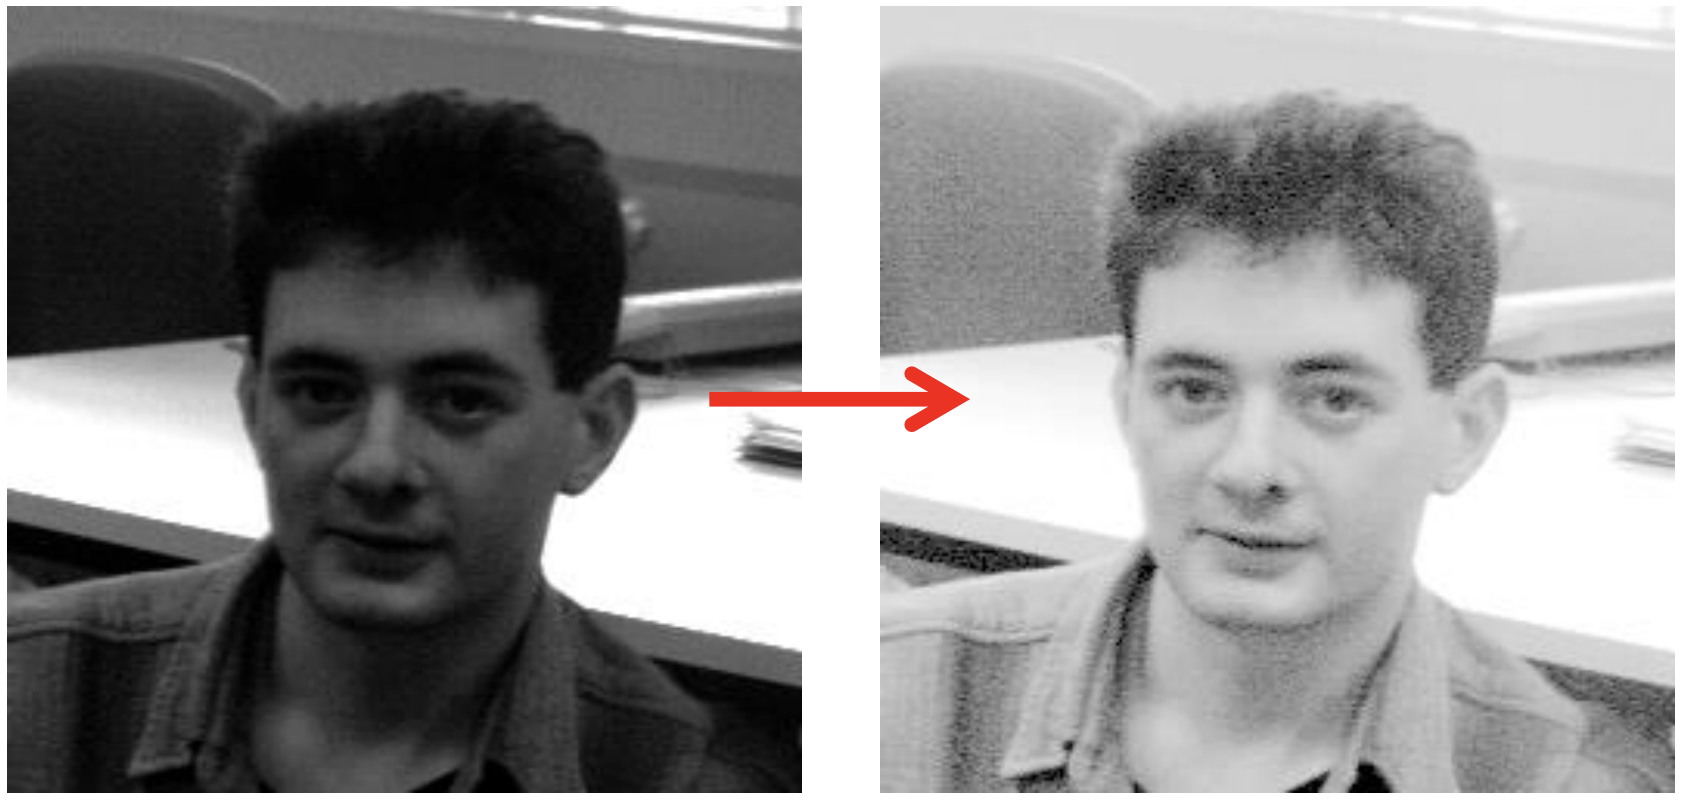
\includegraphics[width=0.8\linewidth]{images/log-transform-1.png}
    \caption{An example of a logarithmic transform applied to increase the dynamic range of the dark parts and decrease the dynamic range in lighter parts.}
    \label{fig:log-transform-1}
\end{figure}

\begin{figure}
    \centering
    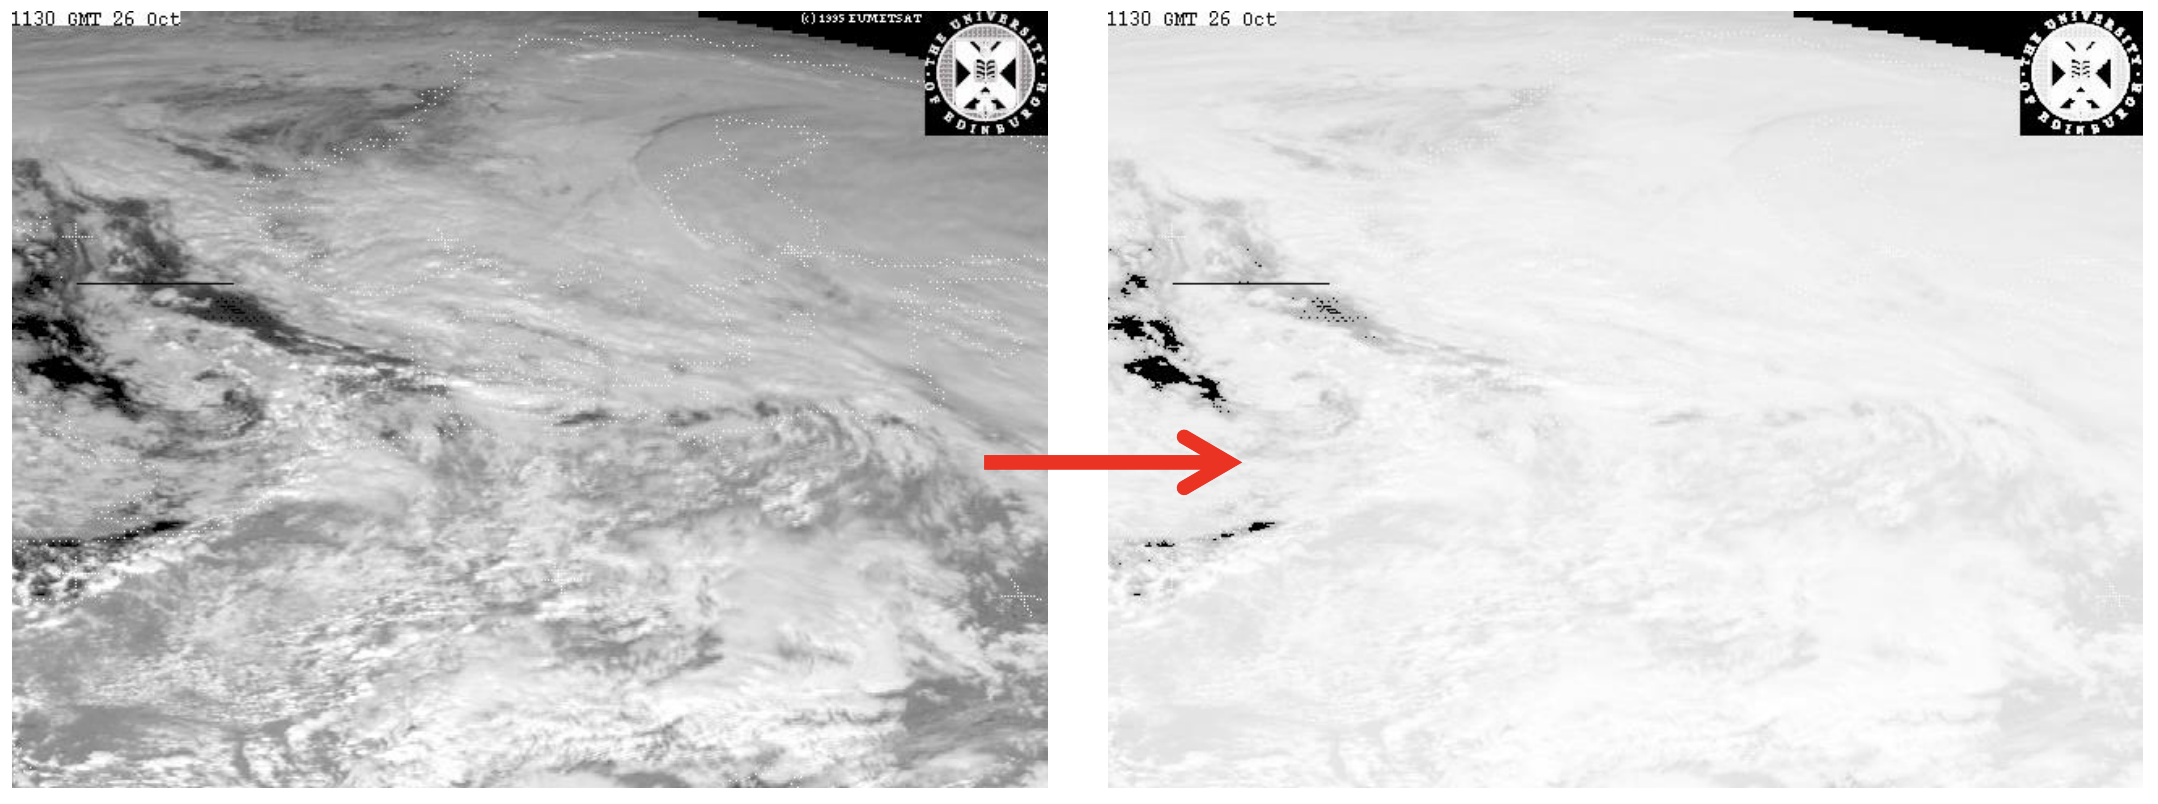
\includegraphics[width=0.8\linewidth]{images/log-transform-2.png}
    \caption{An example showing that applying logarithmic transforms to predominately bright images causes a loss of information.}
    \label{fig:log-transform-2}
\end{figure}

\begin{example}[X-ray images]
    X-ray sensors return an intensity value given 
    $\exp{p}$ 
    where $p$ is the actual intensity of the source.
    Hence, we can use a logarithmic transform to cancel this out
    and give a linear mapping to the intensities.
\end{example}

\section{Exponential transform}

The exponential transform is the inverse of the logarithmic transform (as you would expect), we have:
\[ I_o(i, j) = \exp(I_i(i, j)) \]
and again in practice we typically use parameters $\alpha, c > 0$:
\[ I_o(i, j) = c ((1 + \alpha)^{I_i(i, j)} - 1) \]
where 
$1 + \alpha$ 
is our basis and $c$ is a scaling factor (as before).

\begin{figure}
    \centering
    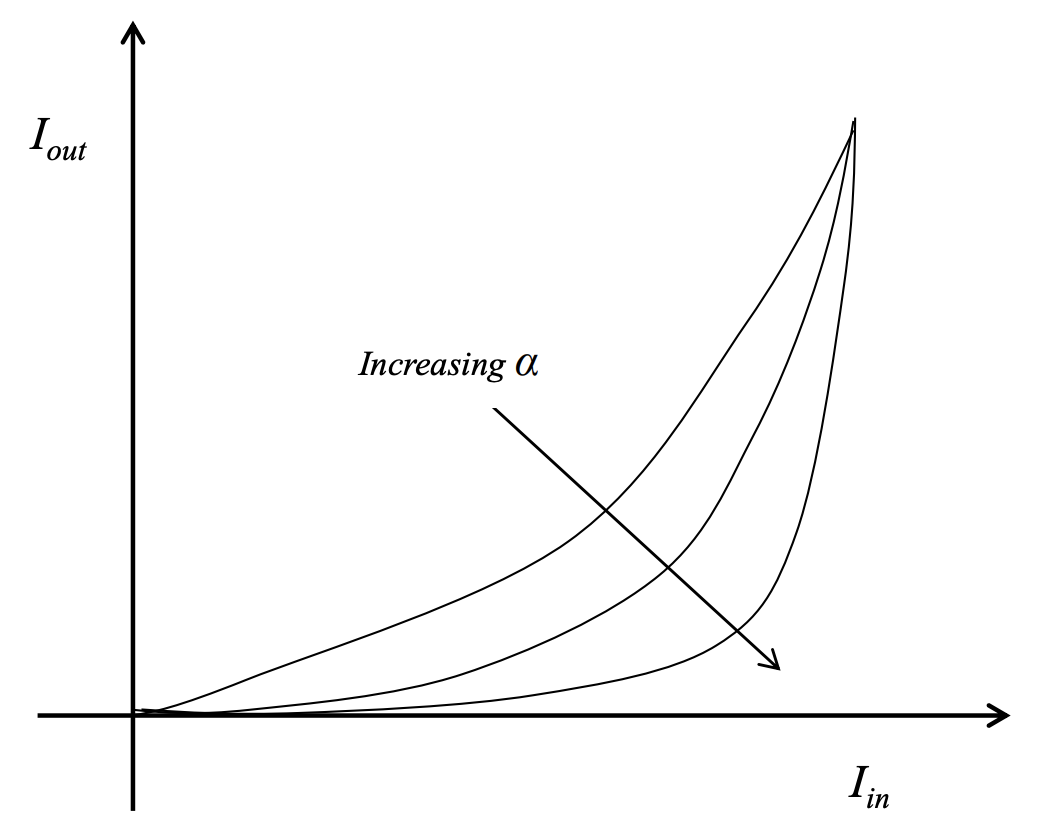
\includegraphics[width=0.5\linewidth]{images/exp-scaling-factor.png}
    \caption{An graph demonstrating how a change in $\alpha$ affects the exponential transform.}
    \label{fig:exp-scaling-factor}
\end{figure}

As predicted, the exponential transform does the opposite to the logarthmic transform.

\begin{figure}
    \centering
    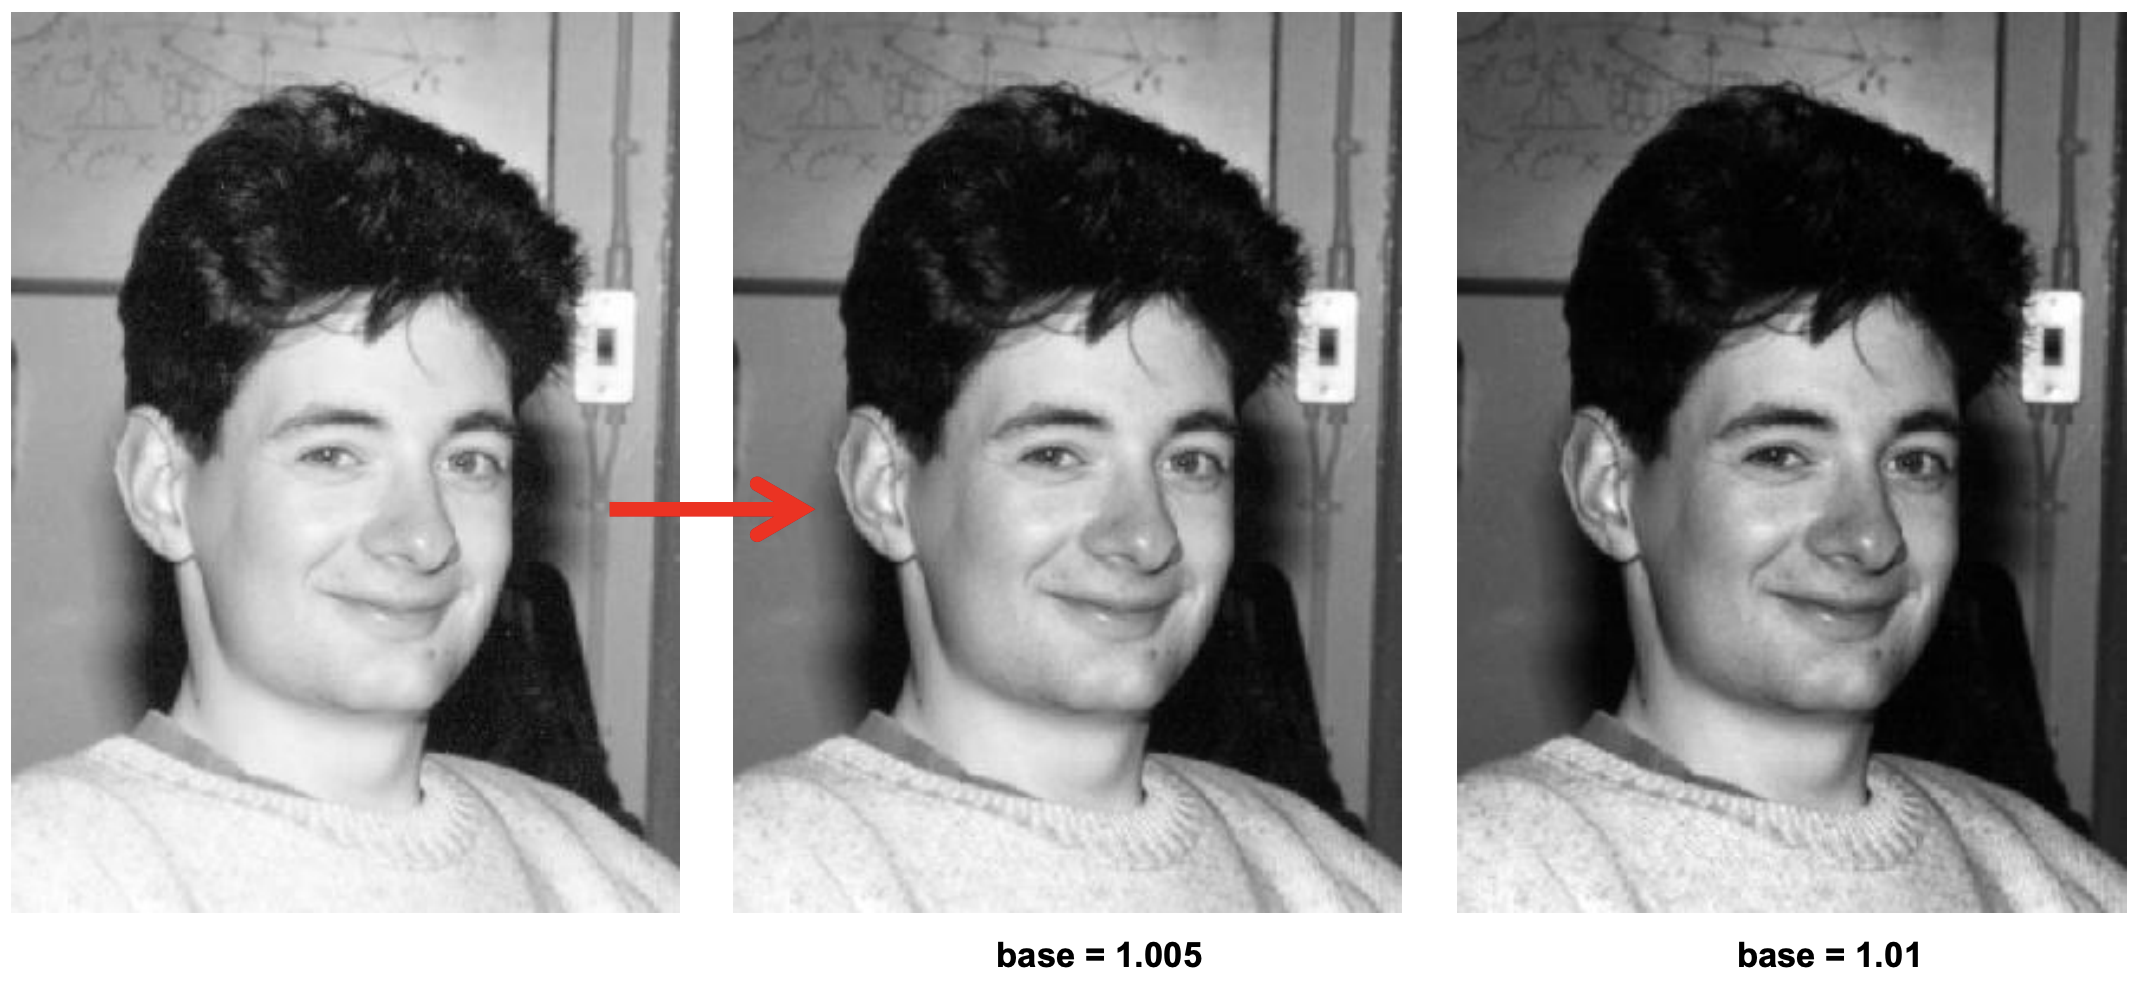
\includegraphics[width=0.8\linewidth]{images/exp-transform.png}
    \caption{An example of an exponetial transform applied to an image with a base of $1.005$ and a base of $1.01$.}
    \label{fig:exp-transform}
\end{figure}

\section{Power-law transform}

The \textbf{power-law transform} is where we raise each pixel to a fixed power
(the normalise with a factor),
so:
\[ I_o(i, j) = c\left(I_i(i, j)\right)^r. \]
If we have $r < 1$: it spreads low intensities and compresses high intensities, much like $\exp$.
If we have $r > 1$: it spreads high intensities and compresses low intensities, much like $\log$.

\begin{figure}
    \centering
    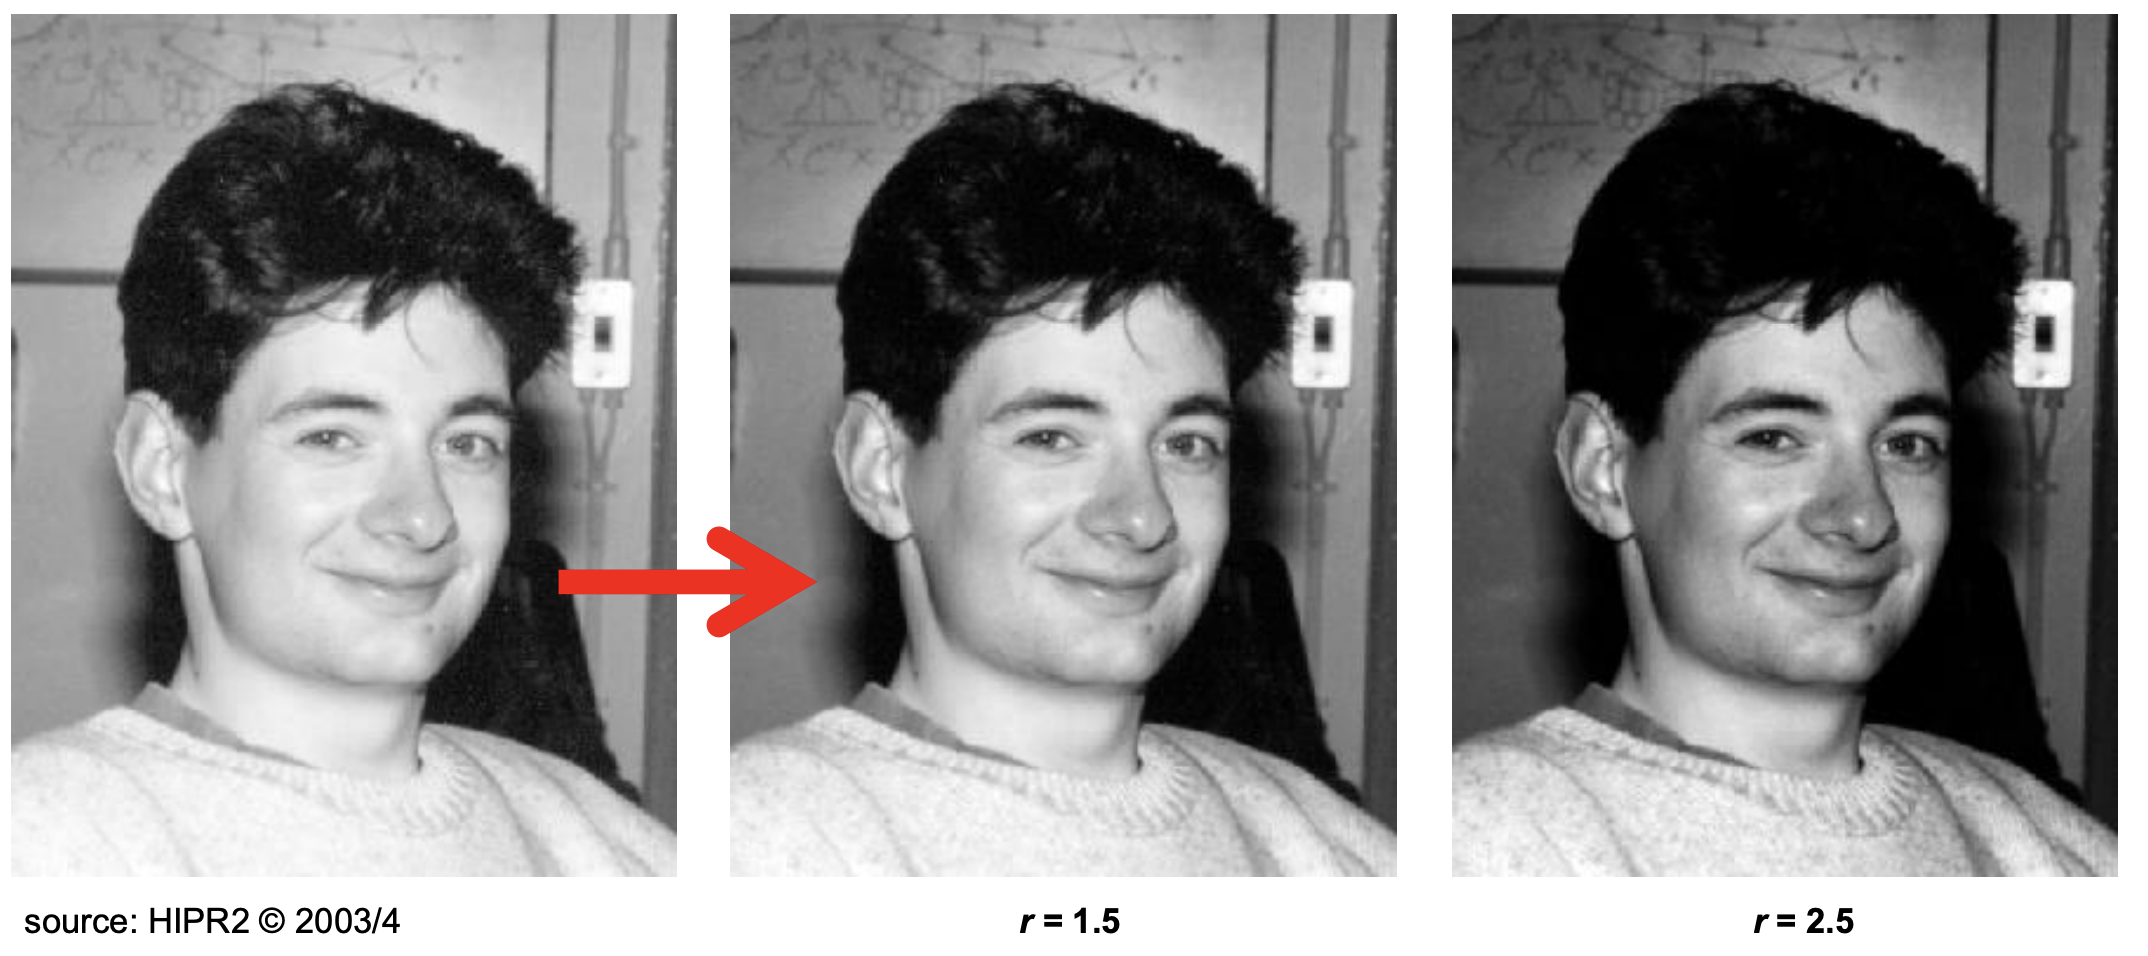
\includegraphics[width=0.8\linewidth]{images/power-law-transform.png}
    \caption{An example of a power-law transform for  $r = 1.5$ and $r = 2.5$.}
    \label{fig:power-law-transform}
\end{figure}

Power-law transforms are typically used in digital photograph to correct the \emph{tonality} of images.
$r$ is typically called the gamma value, and the proccess is called 
\textbf{gamma correction}.

\begin{example}
    \begin{enumerate}
        \item An underexposed photo can be corrected using gamma correction with $\gamma < 1$.
        \item An overexposed photo can be corrected using gamma correction with $\gamma > 1$.
    \end{enumerate}
\end{example}

\begin{figure}
    \centering
    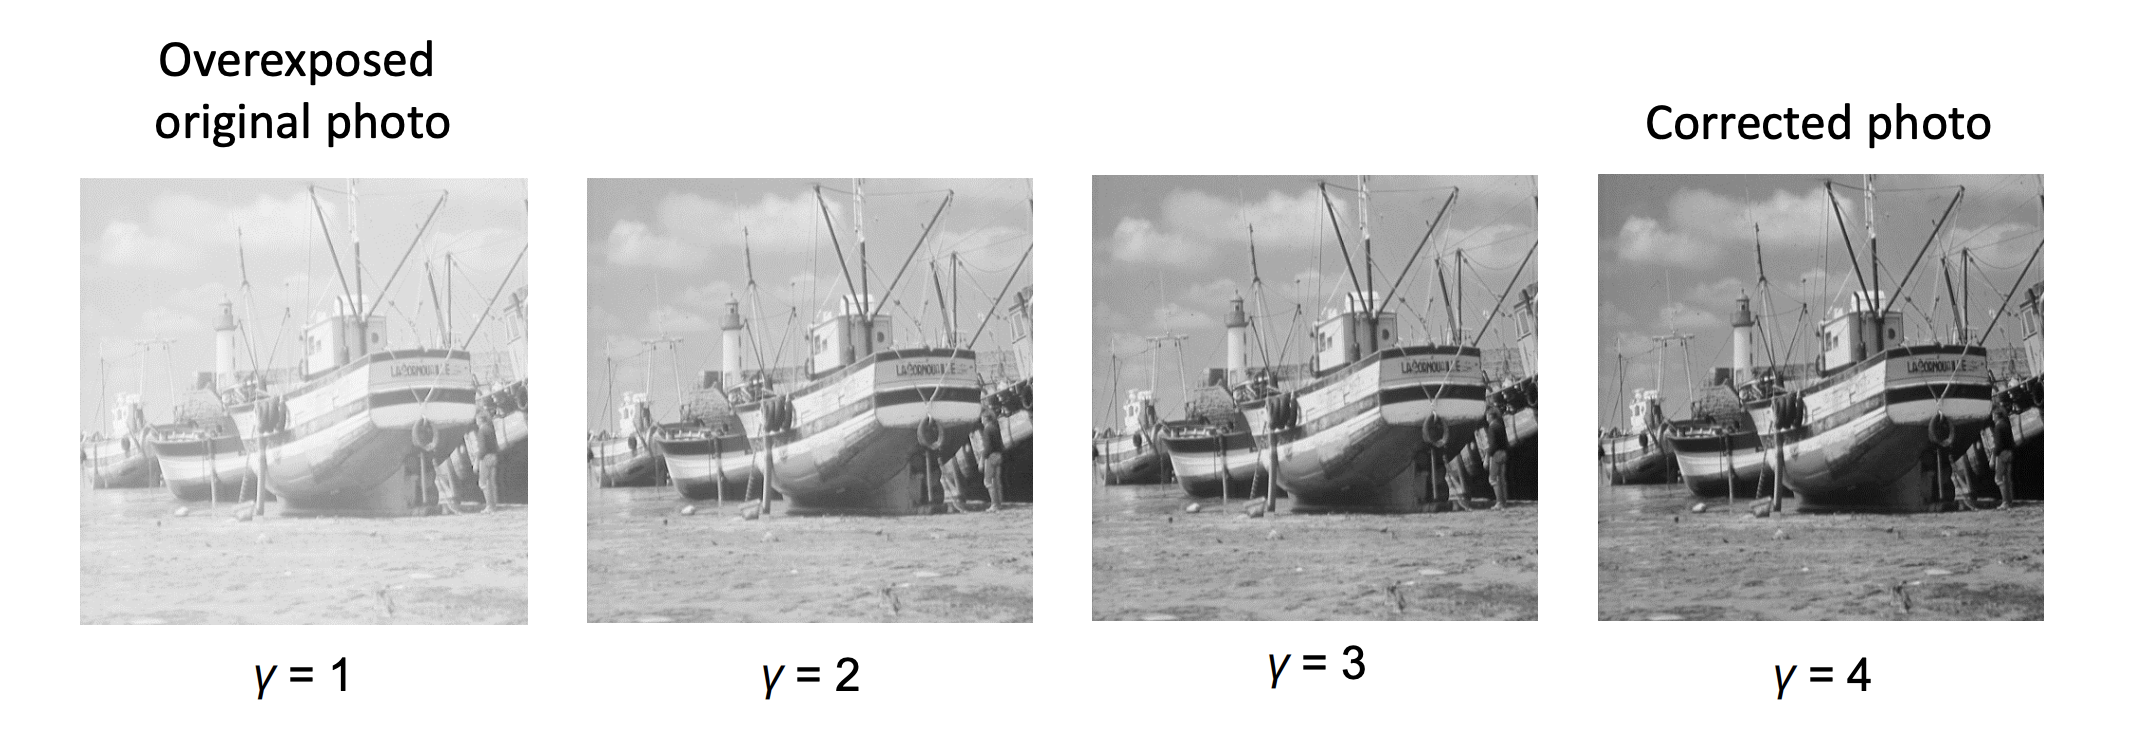
\includegraphics[width=0.8\linewidth]{images/gamma-correction-1.png}
    \caption{An example of gamma correction applied to an overexposed photo.}
    \label{fig:gamma-correction-1}
\end{figure}

\begin{figure}
    \centering
    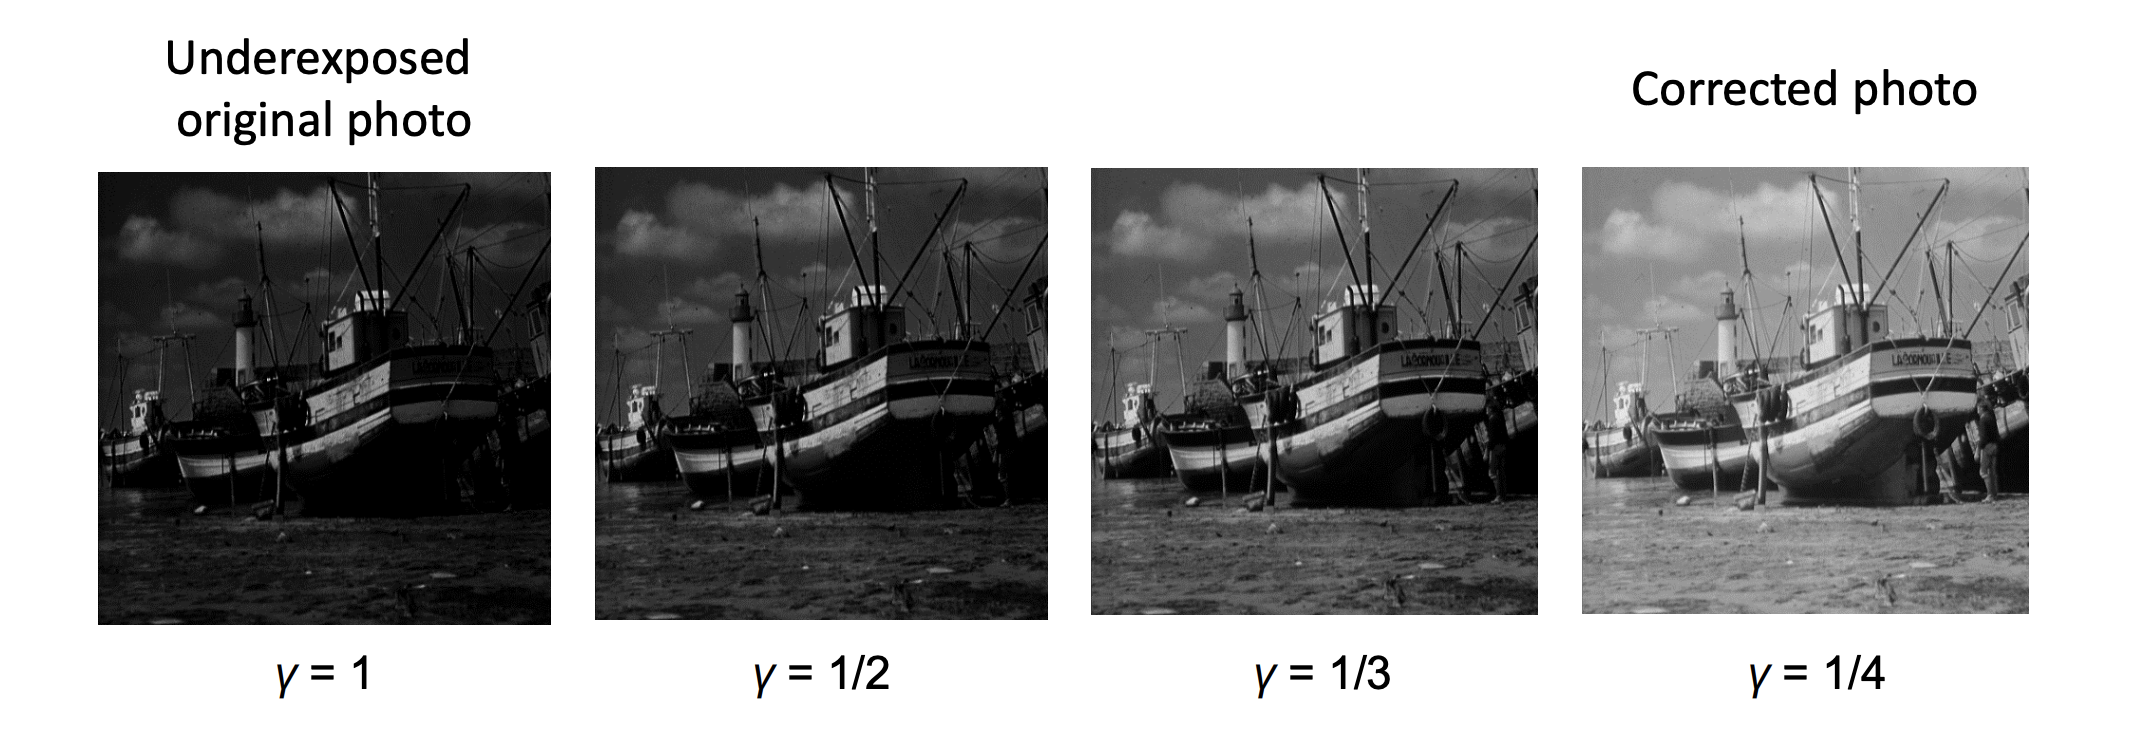
\includegraphics[width=0.8\linewidth]{images/gamma-correction-2.png}
    \caption{An example of gamma correction applied to an underexposed photo.}
    \label{fig:gamma-correction-2}
\end{figure}
